\documentclass[letterpaper, reqno,11pt]{article}
\usepackage[margin=1.0in]{geometry}
\usepackage{color,latexsym,amsmath,amssymb,graphicx, float}
\usepackage{hyperref}

\hypersetup{
colorlinks=true,
linkcolor=magenta,
filecolor=magenta,
urlcolor=cyan,
}

\graphicspath{ {images/} }

\begin{document}
\pagenumbering{arabic}
\title{PHYS 304 Homework 5}
\date{28/02/22}
\author{Xander Naumenko}
\maketitle

{\noindent\bf Question 1.} Starting from a similar point as in the textbook, we are looking for solutions then in the form of
\[
\psi(x)=\begin{cases}
    Fe^{-\kappa x},&(x>a),\\
    D\sin(lx),&(0<x<a),\\
    -\psi(-x),&(x<0).
\end{cases}
\]

The continuity at $x=a$ for both $\psi$ and its derivative gives
\[
Fe^{-\kappa a}=D\sin(la), -\kappa Fe^{-\kappa a}=lD\cos(la)
\]
\[
\implies \kappa=-l\cot(la)
.\]
Defining $z$ and $z_0$ as in the textbook, this formula becomes
\[
\cot z=-\sqrt{(z_0 /z)^2-1} 
.\]
This is the transcendental equation analogous to the one we found for the even states. A graph of the solutions can be seen in figure \ref{fig:q1}. 

\begin{figure}[htpb]
    \centering
    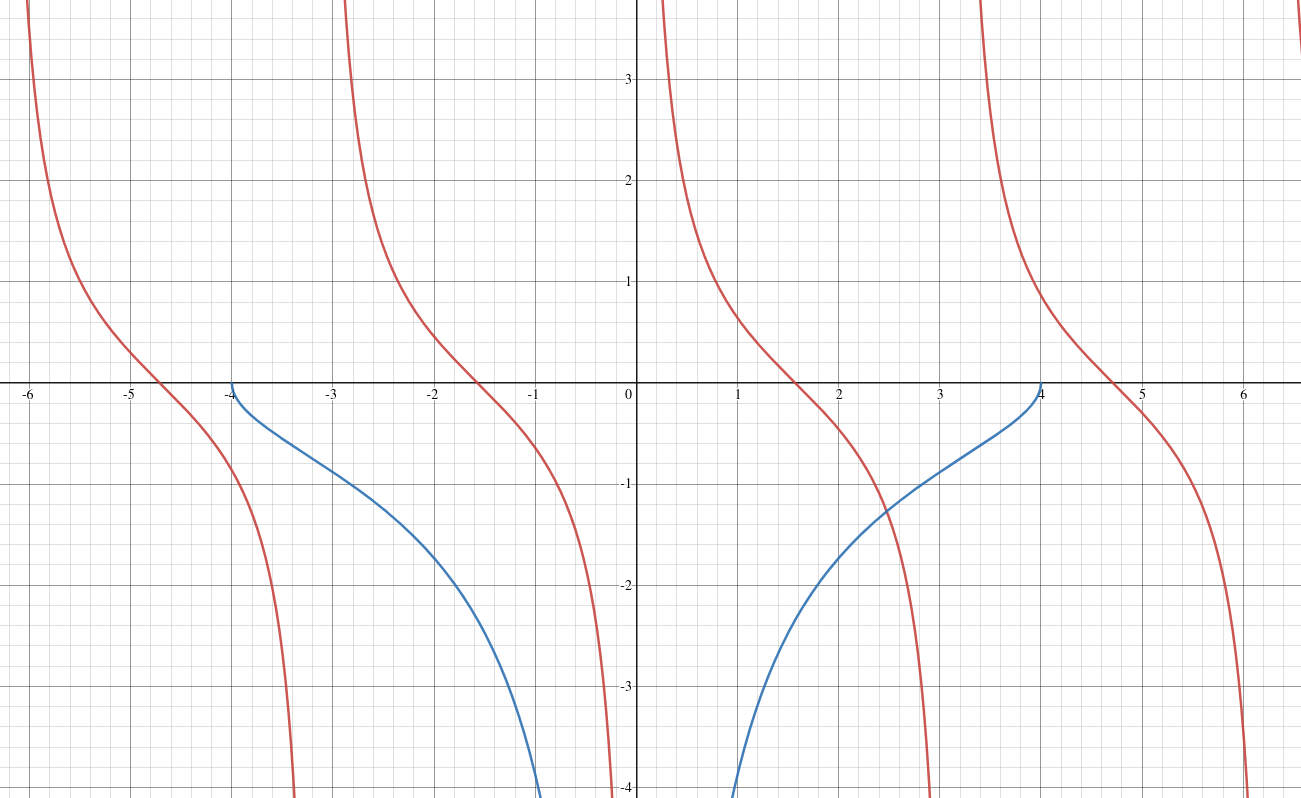
\includegraphics[width=0.8\textwidth]{q1}
    \caption{Graph of the transcendental equation needed to solve the odd bound states. }
    \label{fig:q1}
\end{figure}

For the limiting cases, if the well is deep and wide (i.e. $z_0$ is large) then there are solutions approximately at every multiple $\pi$. In the other case, when $z_0$ is small, there are no odd bound states since there is no intersection between the two equations.

{\noindent\bf Question 2.} First consider the case when $E>V_0$. In this case the analysis is exactly the same as for the potential well, except now we instead define $l$ as 
\[
l=\frac{\sqrt{2m(E-V_0)} }{\hbar}
.\]
Since $E-V_0$ is positive, the analysis proceeds the exact same and for this case the transmission coefficient turns out to be 
\[
T^{-1}=1+\frac{v_0^2}{4E(E+V_0)}\sin^2\left( \frac{2a}{\hbar}\sqrt{2m(E+V_0)}  \right) 
.\]

For the second case, consider when $E+V_0$. In this case the left and right parts of the analysis remain the same, but for in the potential barrier schr\"oedinger's equation reads
\[
\frac{d^2\psi}{dx^2}=0\implies \psi=Cx+D
.\]
Using the boundary conditions, this gives the following set of equations:
\[
Ae^{-ka}+Be^{ika}=D-Cx
.\]
\[
Fe^{ika}=Cx+D
.\]
\[
ik(Ae^{-ka}-Be^{ika})=C
.\]
\[
ikFe^{ika}=C
.\]
Solving these gives that
\[
T^{-1}=\frac{2mE}{\hbar^2}a^2+1
.\]

For the final case for when $E<V_0$, the analysis is similar to the well case except now the sign in front of  $l$ has changed, as has the sign of $V_0$:
\[
\frac{d^2\psi}{dx^2}=l^2\psi, l=\frac{\sqrt{2m(V_0-E)} }{\hbar}
.\]
\[
\implies\psi=Ce^{lx}+De^{-lx}
.\]
This gives us the following equations from the boundary conditions:
\[
Ae^{-ika}+Be^{ika}=Ce^{-la}+De^{la}
.\]
\[
ik\left( Ae^{-ika}+Be^{ika} \right)=l\left( Ce^{-la}+De^{la} \right) 
.\]
\[
Ce^{la}+De^{-la}=Fe^{ika}
.\]
\[
l\left( Ce^{la}-De^{-la} \right) =ikFe^{ika}
.\]
Solving these gives the following result for the transmission coefficient: 
\[
T^{-1}1+\frac{V_0^2}{4E(V_0-E)}\sinh^2\left( \frac{2a}{\hbar}\sqrt{2m(V_0-E)}  \right) 
.\]

{\noindent\bf Question 3a.} This is extremely similar to the finite well case. For $x<0$, the Schr\"odinger equation reads
\[
\frac{d^2\psi}{dx^2}=k^2\psi\implies \psi=Ae^{ikx}+Be^{-ikx}
.\]
To the right it is instead:
\[
\frac{d^2\psi}{dx^2}=l^2\psi, l=\frac{\sqrt{2m(V_0-E)} }{\hbar}
.\]
\[
\implies \psi=Fe^{-lx}
.\]
Applying the boundary conditions we get:
\[
A+B=F, ik(A-B)=-lF
.\]
\[
\implies A+B=-\frac{k}{il}(A-B)\implies B\left( \frac{k}{il}-1 \right) =A\left( 1+\frac{k}{il} \right) 
.\]
\[
\implies R=\left| \frac{B}{A} \right|^2=\frac{\left| \frac{k}{il}+1 \right|^2}{\left| \frac{k}{il}-1 \right|^2}=1
.\]

{\noindent\bf Question 3b.} If $E>V_0$ then $l$ in the previous part has a negative in front of it for the Schr\"odinger equation, which means that for $x>0$, the wavefunction is
\[
\psi=Fe^{ilx}, l=\frac{\sqrt{2m(E-V_0)} }{\hbar}
.\]
Again we can apply the continuity equations to get:
\[
A+B=F, ik(A-B)=ilF
.\]
\[
\implies B\left( \frac{k}{l}+1 \right) =A\left( 1-\frac{k}{l} \right) 
.\]
\[
R=\left| \frac{B}{A} \right| ^2=\frac{|1-\frac{k}{l}|^2}{|\frac{k}{l}+1|^2}=\frac{(l-k)^2}{(l+k)^2}
.\]
where $l$ is as defined above for this question and $k=\frac{\sqrt{2mE} }{\hbar}$. We can also expand in terms of $E$ and $ V_0$ to get
\[
R=\frac{\left( \sqrt{E} -\sqrt{E-V_0}  \right)^{4} }{V_0^2}
.\]

{\noindent\bf Question 4c.} From equation 2.99, we have that  $v_{\text{quantum}}=\sqrt{\frac{2E}{m}} $. On the right side of the step potential though the relative energy in the equation is actually $E-V_0$. Thus across the step the velocity decrease by a factor or $\sqrt{\frac{E-V_0}{E}} $. Logically the "amount" of probability going in either direction is proportional to the magnitude of the wavefunction squared times the velocity, so the numerator of the traditional transmission coefficient also goes down by the same factor and we have
\[
T=\sqrt{\frac{E-V_0}{E}} \frac{|F|^2}{|A|^2}
.\]

{\noindent\bf Question 3d.} Going back to our derived continuity equations, this gives us: 
\[
F-B=\frac{l}{k}F+B\implies F(1+\frac{l}{k})=2B\implies F=\frac{2k}{l+k}B
.\]
\[
\implies T=\left| \frac{F}{A} \right| ^2\sqrt{\frac{E-V_0}{E}}=\frac{4k^2l(k-l)^2}{(k^2-l^2)^2}\sqrt{\frac{E-V_0}{E}}
.\]
Expanding in terms of the energies we have that 
\[
T=\frac{4\sqrt{E} \sqrt{E-V_0}\left( \sqrt{E} -\sqrt{E-V_0}  \right)^2 }{V_0^2}
.\]
Checking, we get that
\[
T+R=\frac{\left( \sqrt{E} -\sqrt{E-V_0}  \right)^{4} }{V_0^2}+\frac{4\sqrt{E} \sqrt{E-V_0}\left( \sqrt{E} -\sqrt{E-V_0}  \right)^2 }{V_0^2}=1
.\]

{\noindent\bf Question 4a.} 

\[
    A+B=\begin{pmatrix} 1&1&0\\2&1&3\\3i&3-2i&4 \end{pmatrix} 
.\]

{\noindent\bf Question 4b.} 

\[
    AB=\begin{pmatrix} -3&1+3i&3i\\4+3i&9&6-2i\\6i&6-2i&6 \end{pmatrix} 
.\]

{\noindent\bf Question 4c.} 

\[
    [A,B]=AB-BA=\begin{pmatrix} -3&1+3i&3i\\4+3i&9&6-2i\\6i&6-2i&6 \end{pmatrix}-\begin{pmatrix} 0&0&0\\2&0&3\\6+3i&-3i&12 \end{pmatrix}=\begin{pmatrix} -3&1+3i&3i\\2+3i&9&3-2i\\-6+3i&6+i&-6 \end{pmatrix} 
.\]

{\noindent\bf Question 4d.} 

\[
    \tilde A=\begin{pmatrix} -1&2&2i\\1&0&-2i\\i&3&2 \end{pmatrix} 
.\]

{\noindent\bf Question 4e.} 

\[
    A^*=\begin{pmatrix} -1&1&-i\\2&0&3\\-2i&2i&2 \end{pmatrix} 
.\]

{\noindent\bf Question 4f.} 

\[
    A^\dagger=\begin{pmatrix} -1&2&-2i\\1&0&2i\\-i&3&2 \end{pmatrix} 
.\]

{\noindent\bf Question 4g.} 

\[
\det(B)=2\cdot 1\cdot 2-i(-i)=4-1=3
.\]

{\noindent\bf Question 4h.} Row reducing: 

\[
    \begin{pmatrix} 2&0&-i&1&0&0\\0&1&0&0&1&0\\i&3&2&0&0&1 \end{pmatrix} \implies \begin{pmatrix} 1&0&-\frac{i}{2}&\frac{1}{2}&0&0\\0&1&0&0&1&0\\0&0&\frac{3}{2}&-\frac{i}{2}&-3&1 \end{pmatrix} 
.\]

\[
    \implies B^{-1}=\begin{pmatrix} \frac{2}{3}&-i&\frac{i}{3}\\0&1&0\\-\frac{i}{3}&-2&\frac{2}{3} \end{pmatrix} 
.\]
Checking:
\[
    BB^{-1}=\begin{pmatrix} 2&0&-i\\0&1&0\\i&3&2 \end{pmatrix}\begin{pmatrix} \frac{2}{3}&-i&\frac{i}{3}\\0&1&0\\-\frac{i}{3}&-2&\frac{2}{3} \end{pmatrix}=\begin{pmatrix} 1&0&0\\0&1&0\\0&0&1 \end{pmatrix} 
.\]
As for $A$, we can calculate its determinant: 
\[
\det A=-1(-2i)(-3)-(4-6i)+i(-4i)=0
.\]
Therefore $A$ doesn't have an inverse. 

\end{document}
